\begin{abstract}
Random forests (RF) and deep networks (DN) are two of the most popular machine learning methods in the current scientific literature and yield differing levels of performance on different data modalities. We wish to further explore and establish the conditions and domains in which each approach excels, particularly in the context of sample size and feature dimension. To address these issues, we tested the performance of these approaches across tabular, image, and audio settings using varying model parameters and architectures.
Our focus is on datasets with at most 10,000 samples, which represent a large fraction of scientific and biomedical datasets.
In general, we found RF to excel at tabular and structured data (image and audio) with small sample sizes, whereas DN performed better on structured data with larger sample sizes. Although we plan to continue updating this technical report in the coming months, we believe the current preliminary results may be of interest to others.
\end{abstract}

\section{Introduction}
Random forests (RF) and deep networks (DN) have gained prominence in the scientific literature as two of the highest performing techniques for machine learning tasks, including classification. RF methods have dominated tabular data scenarios, where the relative position of features is irrelevant. Their dominance includes high performance on real-world tabular data tasks and machine learning competitions, demonstrating their relevance to the many biomedical applications represented by tabular data \citep{Wager2017-qk, microarray, spectral, svetnik}. In contrast, DN dominates structured data scenarios, where the relative position of features is key for sample identification. Those include image, audio, and text data, where feature position can be extracted from DN layers using convolutions and other metrics \citep{Krizhevsky2012-sq, Zhang2020-vg, Brown2020-tz, resnet}.

The ``arbitrary slow convergence'' theorem and the ``no free lunch'' theorem prove that no one approach can outperform another approach in all problems \citep{slow_conv, lunch}. While RF and DN are commonly studied to determine their optimal usage, we aimed to compare them directly and establish the general domain parameters in which each model performs best. To achieve this objective, we used three data modalities: tabular, image, and audio, and varied training set sample sizes for each dataset.
By understanding the inherent bias-variance trade-off and its impact on numerous data sources, we aimed to lay out the regions of problem space where each approach outperforms the other.
Using these datasets, we outlined findings in each domain under practical data applications.

\section{Tabular}
\label{tabular}
We used OpenML-CC18 for tabular benchmarks, which is a collection of 72 datasets organized by OpenML to function as a comprehensive benchmark suite \citep{OpenML2013, bischl}. These datasets vary in sample size, feature space, and unique target classes.
About half of the datasets are binary classification tasks, and the other half are classification tasks with up to 50 classes. The range of total sample sizes of the datasets was between 500 and 100,000, while the range of features was from a few to a few thousand.
Datasets were imported using the OpenML python package, which is BSD-licensed \citep{OpenMLPython2019}.

\subsection{Methods}
\subsubsection{Computing}
All datasets with over 10,000 samples were randomly downsampled to 10,000 samples. Next, for each dataset, the training data were indexed into eight subsets with evenly spaced sample sizes on a logarithmic scale, thus producing eight training sets with different sample sizes. The smallest of these sample sizes had five times the number of classes in the dataset, and the largest sample size used the entire dataset.
Evaluation of each of these training sets was performed using 5-fold cross-validation, with the held-out test fold used to evaluate all sample sizes for the given dataset.

Random forest is a non-parametric and universally consistent estimator, so it will approach Bayes optimal performance with sufficiently large sample sizes, tree depths, and trees \citep{biau}.
We used 500 trees with no depth limit, only varying the number of features selected per split (``max-features'').
Letting $d$ equal the number of features in the dataset, we varied max-features to be one of: $\sqrt{d}$, $d/4$, $d/3$, $d/1.5$, and $d$ \citep{parameter}.

For optimizing hyperparameters in a deep network, we essentially followed the guidance of \citet{bouthillier}. This multi-layer perceptron used a single hidden layer from scikit-learn's (BSD 3-Clause) \texttt{MLPClassifier} \citep{scikit-learn}. The default setting was used for weight initialization, and the following parameters were tuned: hidden layer size between 20 and 400, and the L2 regularization parameter along log-uniform from $1 \times 10^{-5}$ to $1 \times 10^{-2}$. These parameters were determined based on previous classification work by \citet{jurtz} on the amino acid dataset \citep{MHC}.
To extend this optimization to over-parametrized deep networks, we also searched over the number of layers of the network from one to three hidden layers spanning all combinations of node sizes from 20 to 400. 

For all hyperparameter tuning in both RF and DN, the tuning was conducted only on the entire dataset, using a randomized hyperparameter search with five folds. Tuned hyperparameters were then consistent for all smaller sample sizes per dataset. All tabular benchmarks were run on a 2.3 GHz 8-core Intel i9 CPU. Model training and hyperparameter tuning were parallelized using all available cores.

\subsubsection{Evaluation Criteria}
Cohen's Kappa ($\kappa = \frac{p_o - p_c}{1 - p_c}$, where $p_o$ is the proportion of agreements, and $p_c$ is the expected proportion of chance agreements) is an evaluation metric between two raters that determines the level of agreement between each \citep{cohen}.
To compare the performance of DN and RF, we subtracted DN's Kappa from RF's Kappa for each dataset at each sample size. Unlike classification accuracy, Cohen's Kappa normalizes its score by accounting for chance accuracy. It can be a powerful tool for this experiment because, at small sample sizes, chance accuracy may have a large impact on the model evaluation. In the case of supervised classification, the two raters represent the predictions of the machine learning models and the ground truth of the data. The mean Kappa value was then recorded across the five folds for every sample size. A higher number represents higher accuracy, where a perfectly accurate model has a Kappa of one.

Expected calibration error (ECE) is a metric used to compare two distributions by calculating the expected difference between accuracy and confidence. In addition to Cohen's Kappa, ECE was computed for each dataset, and comparison was calculated by subtracting DN's ECE from RF's ECE at each sample size. This method is executed by storing predictions in $N$ equally spaced bins and calculating the weighted averages of the bins' differences in accuracy versus confidence \citep{pmlr-v70-guo17a}.
A lower number represents higher calibration, where a perfectly calibrated model has an ECE of zero.

Lastly, training wall times were recorded for both models. This metric calculated the fitting time for the given model after hyperparameter tuning, measured in seconds.

\subsection{Results}
\subsubsection{Cohen's Kappa and ECE}
Sample sizes were plotted on a logarithmic scale, whereas Cohen's Kappa and ECE performance were plotted linearly (Figure \ref{fig:tab}). As seen from these results, there is a high level of variability between tabular datasets at each sample size. At larger sample sizes, RF tends to win Cohen's Kappa and excel at accuracy, but DN would win ECE and achieve better calibration.

\subsubsection{Training Wall Times}
Sample size seemed to have little impact on RF training wall times, yet there was an overhead cost of slightly less than one second to fit these models (Figure \ref{fig:tab}). DN, on the other hand, was an order of magnitude faster than RF at small sample sizes, but quickly increased to be an order of magnitude slower as sample size increased.

\begin{figure}[!htb]
\centering
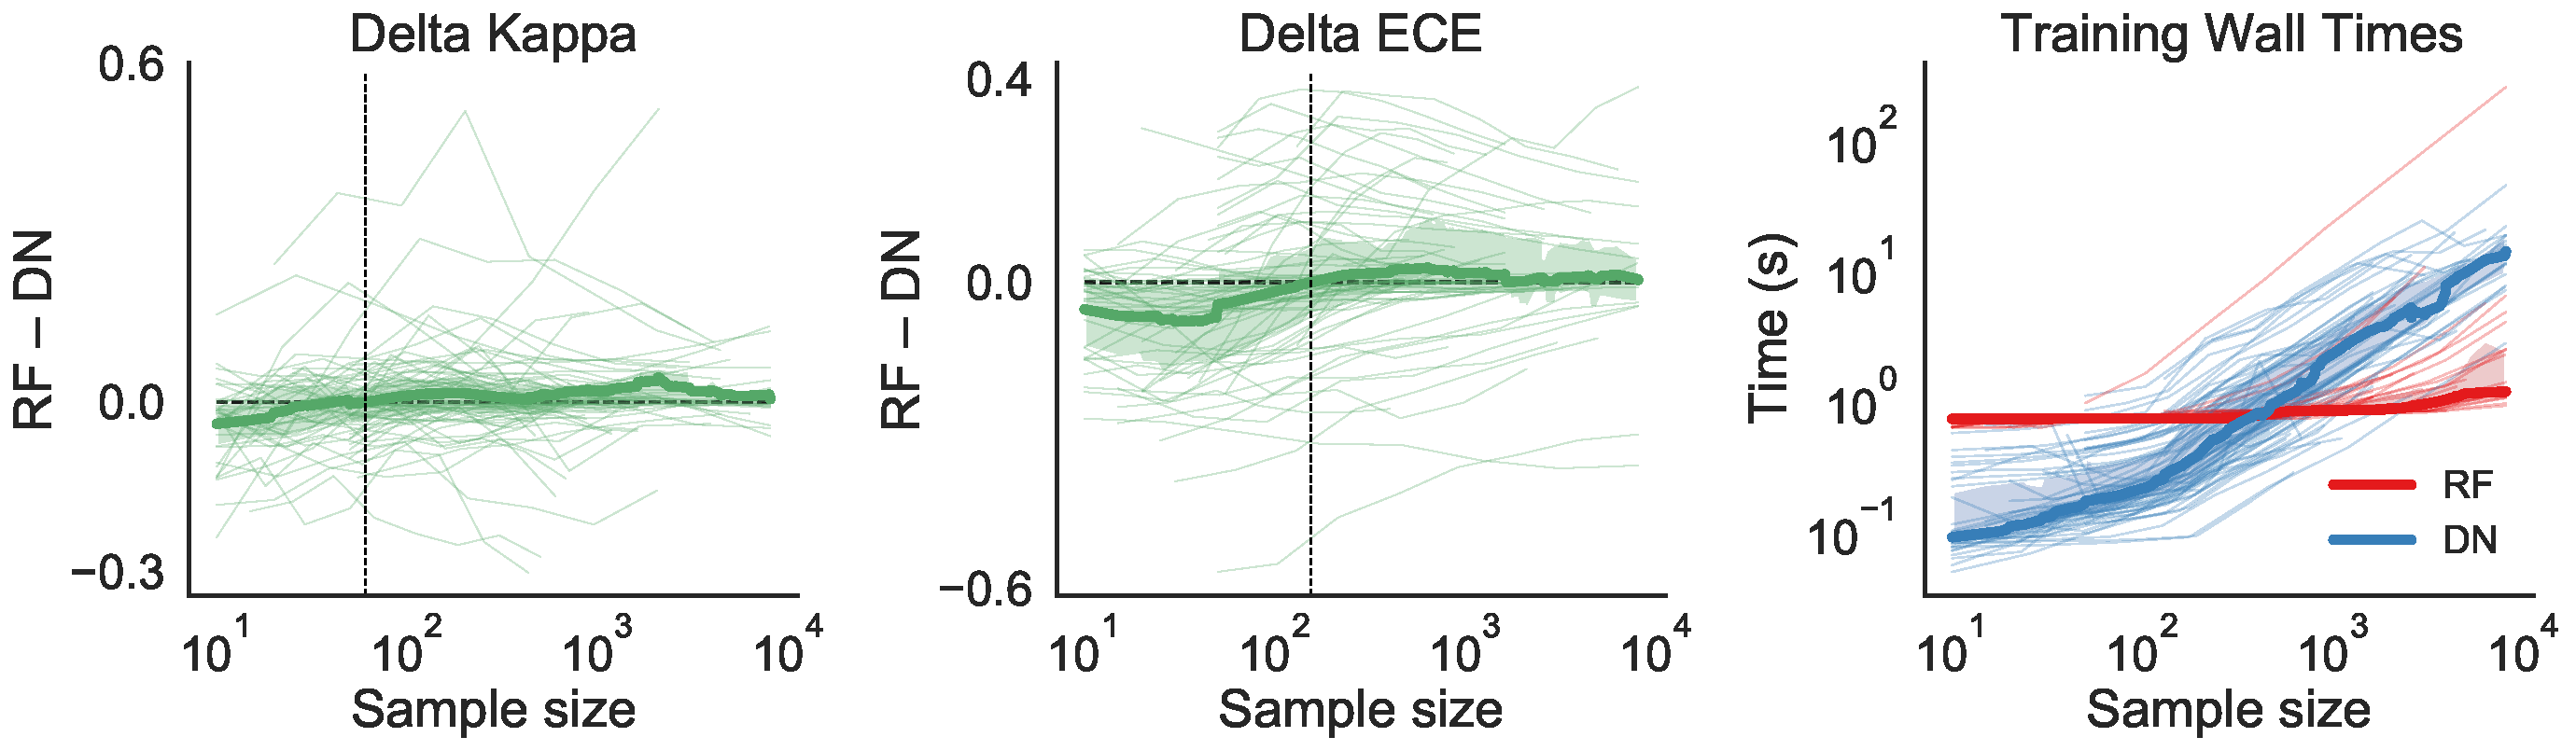
\includegraphics[width=1.0\textwidth]{figures/cc18.pdf}
  \caption{Performance of DN subtracted from performance of RF, evaluated using Cohen's Kappa \textbf{(Left)} and expected calibration error (ECE) \textbf{(Center)}; and training wall times of DN and RF \textbf{(Right)}. 
  For all plots, thin lines represent individual datasets, and shaded regions represent the 25th through 75th percentiles. Left plot represents the difference in Cohen's Kappa versus sample size. Positive values represent better RF performance at the given sample size. Center plot represents the difference in ECE versus sample size. Negative values represent better calibration for RF. Thick green lines in both plots represent the interpolated means over all datasets. Right plot shows training wall times versus sample size. Thick lines represent the interpolated medians. 
  Delta Kappa shows that RF is more accurate at larger sample sizes, while Delta ECE suggests that DN is better calibrated at larger sample sizes. For training wall times, DN is faster than RF at lower sample sizes and slower than RF at larger sample sizes.
  }
\label{fig:tab}
\end{figure}
% \vfil\eject

Given the OpenML-CC18 tabular dataset suite, there appears to be little relationship between average model performance and sample size. However, tabular benchmarks (Figure \ref{fig:tab}) did show trends differentiating the classifiers' ECE scores, which suggest that RF could produce better-calibrated models at lower sample sizes. Should model calibration be the priority, this difference yields a framework for selecting the optimal method given the available sample size on general tabular data. The behavior of training wall times also suggests a trade-off for method choices. At larger sample sizes, DN training wall times would scale much faster. If time is a limiting factor, then RF may be the ideal selection for novel tabular data at large sample sizes.

\section{Image}
\label{image}
We used CIFAR-10 and CIFAR-100 datasets to evaluate the performance of DN and RF on image data, primarily because of the number of classes and large sample sizes of these datasets \citep{cifar}.
Each dataset contains 60,000 colored images with 32x32 pixels, which are separated into 10 or 100 classes, resulting in 6,000 or 600 images per class.
We also included the SVHN dataset as a supplement (Appendix \ref{svhn}) \citep{svhn}. 
Each high-dimensional image sample would be represented by RGB pixels and thus contain $32 \times 32 \times 3 = 3,072$ features.

\subsection{Methods}
\subsubsection{Computing}
We experimented with multi-class classifications in 3-class, 8-class, and 90-class settings. We sampled the 3-class and 8-class training sets from the CIFAR-10 and SVHN datasets and the 90-class training sets from the CIFAR-100 dataset. For each classification task, we ensured 45 random combinations of class labels and up to 10,000 training samples, stratifying data equally across the classes.

For classical architectures, we used \texttt{RandomForestClassifier} and \texttt{SVC} (``rbf'' kernel) from the scikit-learn python package \citep{scikit-learn}. For the deep learning models, four convolutional neural network (CNN) architectures using rectified linear unit (ReLU) activation were employed: three simpler models built with varying parameters and ResNet-18 \citep{resnet}. We adapted the pre-trained ResNet-18 classifier from PyTorch (BSD-3) as a robust choice and optimized its last layer with our training sets \citep{pytorch}. Among the three simpler CNNs, the first network is a simple architecture consisting of one convolutional layer of 32 filters with ReLU and one fully connected layer. The second CNN consists of two convolutional layers each with 32 filters and ReLU, followed by two fully connected layers with 100 and 10 nodes, respectively. Lastly, we constructed a CNN with five convolutional layers that scale up to 128 feature maps, and each layer is followed by batch normalization and ReLU. All convolutions end with one or two fully connected layers with ReLU.

For the high-dimensional image data, our main principle of hyperparameter setup is to minimize tuning and benchmark models with their default values ``out of the box.'' For RF and SVM-RBF, we used their default parameters of the scikit-learn library for all model aspects except RF's number of concurrent jobs ran in parallel utilizing all the cores \citep{scikit-learn}. We benchmarked these models on two Microsoft Azure compute instances: a 2-core Standard\_DS2\_v2 (Intel Xeon E5-2673 v3) and a 6-core Standard\_NC6 (Intel Xeon E5-2690 v3) (Table \ref{table:azure}).

\begin{table}[!htb]
\centering
\begin{tabular}{ |c|c|c|c|c|c| } 
\hline
Compute Instance & vCPU & Memory: GiB & SSD: GiB & GPU & GPU Memory: GiB \\
\hline
Standard\_DS2\_v2 & 2 & 7 & 14 & 0 & N/A \\
\hline
Standard\_NC6 & 6 & 56 & 340 & 1 & 12 \\
\hline
\end{tabular}
\caption{Specifications for Azure compute instances.}
\label{table:azure}
\end{table}

We implemented all of our DN models with a learning rate of 0.001 and a batch size of 64, using stochastic gradient descent with a momentum of 0.9 and cross-entropy loss. These hyperparameters were chosen either by default or commonly seen in literature, and for our training iterations, our settings provided the model with enough time to visually converge on the loss \citep{Krizhevsky2012-sq, pmlr-v119-rice20a}.
We first implemented the networks with 30 epochs and activated early stopping when validation loss did not improve in three epochs in a row \citep{li, lutz, caruana}. In these tasks, we randomly selected 30\% of the provided test sets as validation data and only used the held-out 70\% for benchmarks.

Alternative approaches restricted CNN epochs by calibrating their training wall times or money cost, conforming to those of RF as run on different compute instances. The alternative approaches used the full data of the provided test sets for benchmarks. All approaches were benchmarked on the 1-core GPU component of a Microsoft Azure compute instance: Standard\_NC6 (NVIDIA Tesla K80).
We utilized the GPU with the PyTorch CUDA library \citep{pytorch}.

\subsubsection{Evaluation Criteria}
We evaluated the performance by classification accuracy and training wall times. The training wall times calculated the fitting time for the given model after hyperparameter tuning, measured in seconds. The provided test sets were used.

\subsection{Results}
\subsubsection{Unbounded Time and Cost}
The classification accuracy of RF and SVM-RBF were very similar, and SVM-RBF surpassed RF by a small margin at larger sample sizes (Figure \ref{fig:cifar}). Both classifiers outperformed the networks at smaller sample sizes. However, CNN accuracy often overcame that of the classical models eventually. Higher class numbers decreased the accuracy of all models implemented, but the advantages of RF and SVM-RBF at smaller sample sizes also diminished as the number of classes increased. ResNet-18 with early stops completely surpassed both models in the 90-class classification task. Among the neural networks, more convolutional layers produced higher accuracy, and the performance of 5-layer CNN was very close to that of ResNet-18. ResNet-18 always surpassed other models at the maximum sample size.

Although RF and SVM-RBF had similar overall accuracy, SVM-RBF's training wall times quadratically increased with the sample sizes and eventually surpassed all other models' (Figure \ref{fig:cifar}). The training wall times of parallelized RF stayed relatively constant until acquiring faster growths at larger sample sizes. With early stopping, CNNs would produce training time descents at around 100 samples and increase along with sample size again with slower growth rates. The training time trajectories of CNNs partially overlapped each other and always stayed higher than those of RF. Only the 90-class task produced noticeable differences for CNNs' training wall times, which became more visible at larger sample sizes.

\begin{figure}[!htb]
\centering
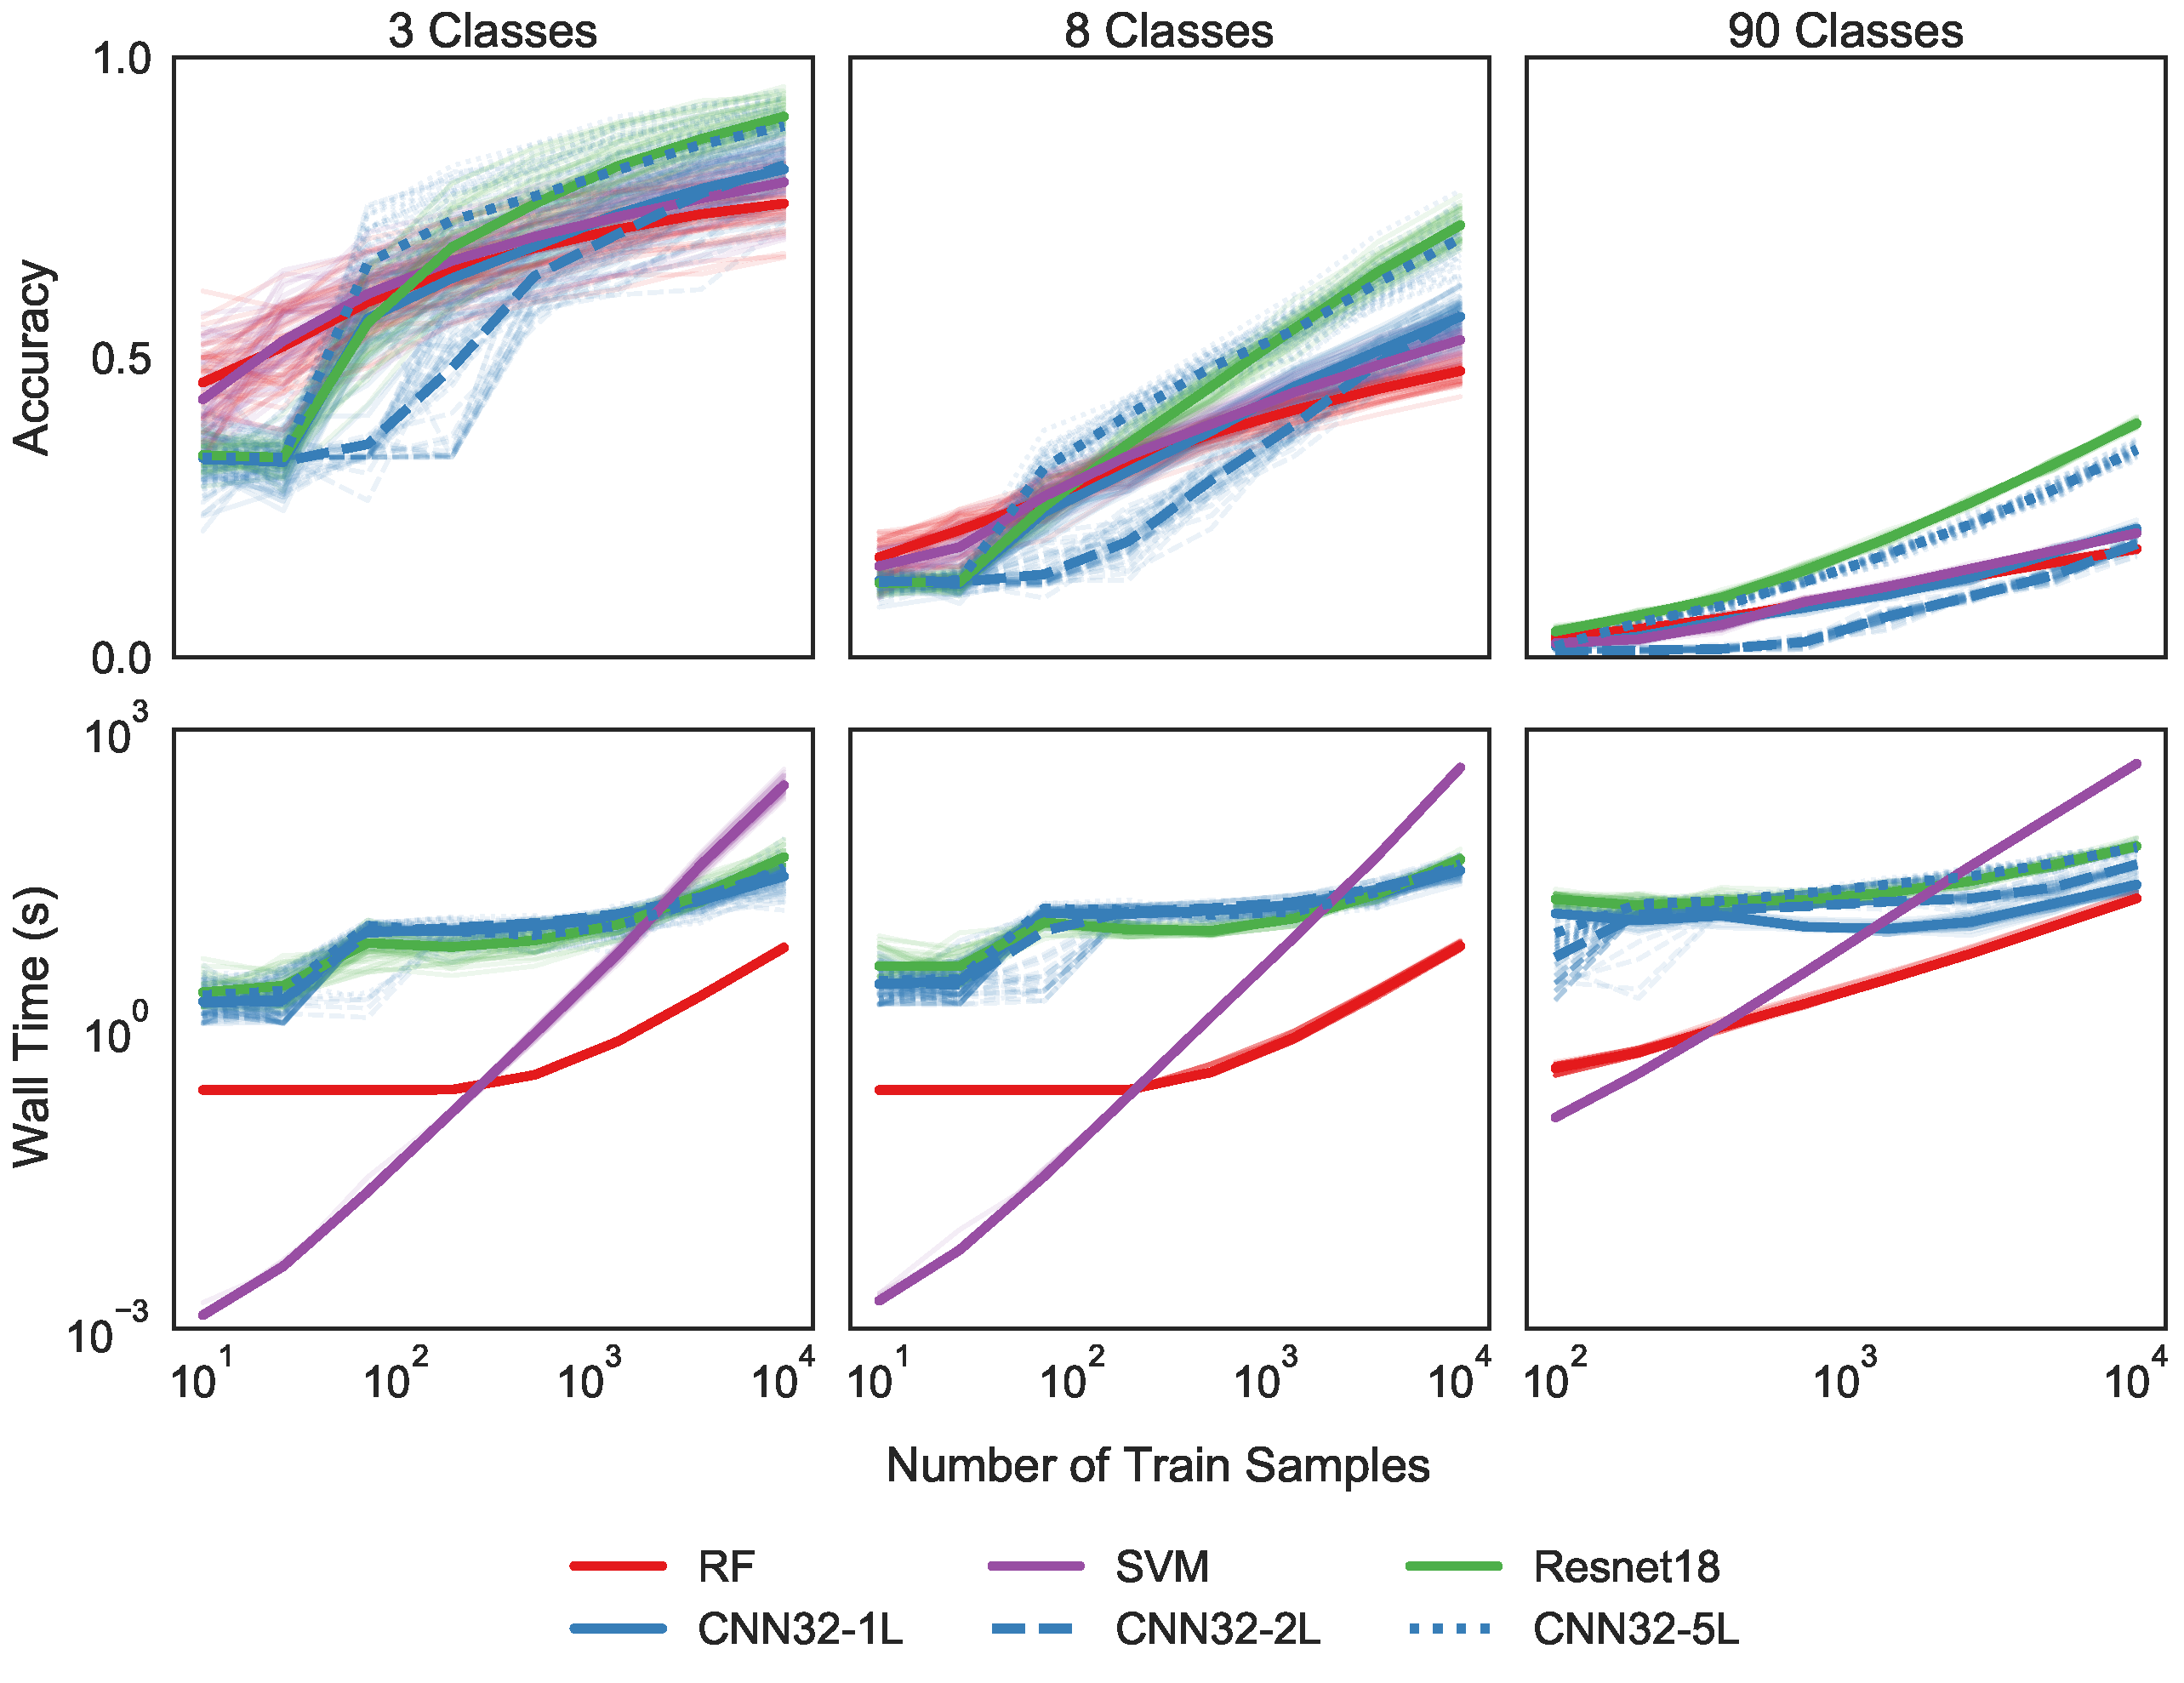
\includegraphics[width=0.8\textwidth]{figures/cifar.pdf}
  \caption{Performance of RF, SVM-RBF, and DN on multiclass CIFAR-10/100 classifications with unbounded time and cost.
  Upper row represents classifier accuracy on a linear scale, and bottom row represents training wall times in seconds on a logarithmic scale. The x-axes correspond to logarithmic sample sizes for respective columns. Each panel shows average results over 45 random combinations. The left two columns use CIFAR-10, while the rightmost uses CIFAR-100.
  Compared to CNNs, RF and SVM-RBF perform better and faster at small sample sizes. While SVM-RBF's training wall times increase quadratically, RF with similar performance is always more efficient than CNNs. As the class number increases, more complex DN has better classification accuracy and longer training wall times.
  }
\label{fig:cifar}
\end{figure}
% \vfil\eject

\subsubsection{Fixed Training Time}
We then compared methods such that each took about the same time on the same virtual machine for 10,000 training samples. The baseline was RF's training times when run on the 6-core Standard\_NC6 Azure compute (Table \ref{table:azure}).
All training wall times except that of SVM-RBF reference conformed to one shape (Figure \ref{fig:cifar_st}). Under the resource constraints, all the accuracy trajectories of CNNs were lower than those in the unbounded benchmarks (Figure \ref{fig:cifar}). Only at around 1,000 samples did CNN accuracy surpass that of RF, whereas 100 samples was the dividing point for benchmarks without restraints. ResNet-18 still had the highest accuracy at the maximum sample size, surpassing all other classifiers eventually. The results with fixed training cost were qualitatively similar (Figure \ref{fig:cifar_sc}).

\begin{figure}[!htb]
\centering
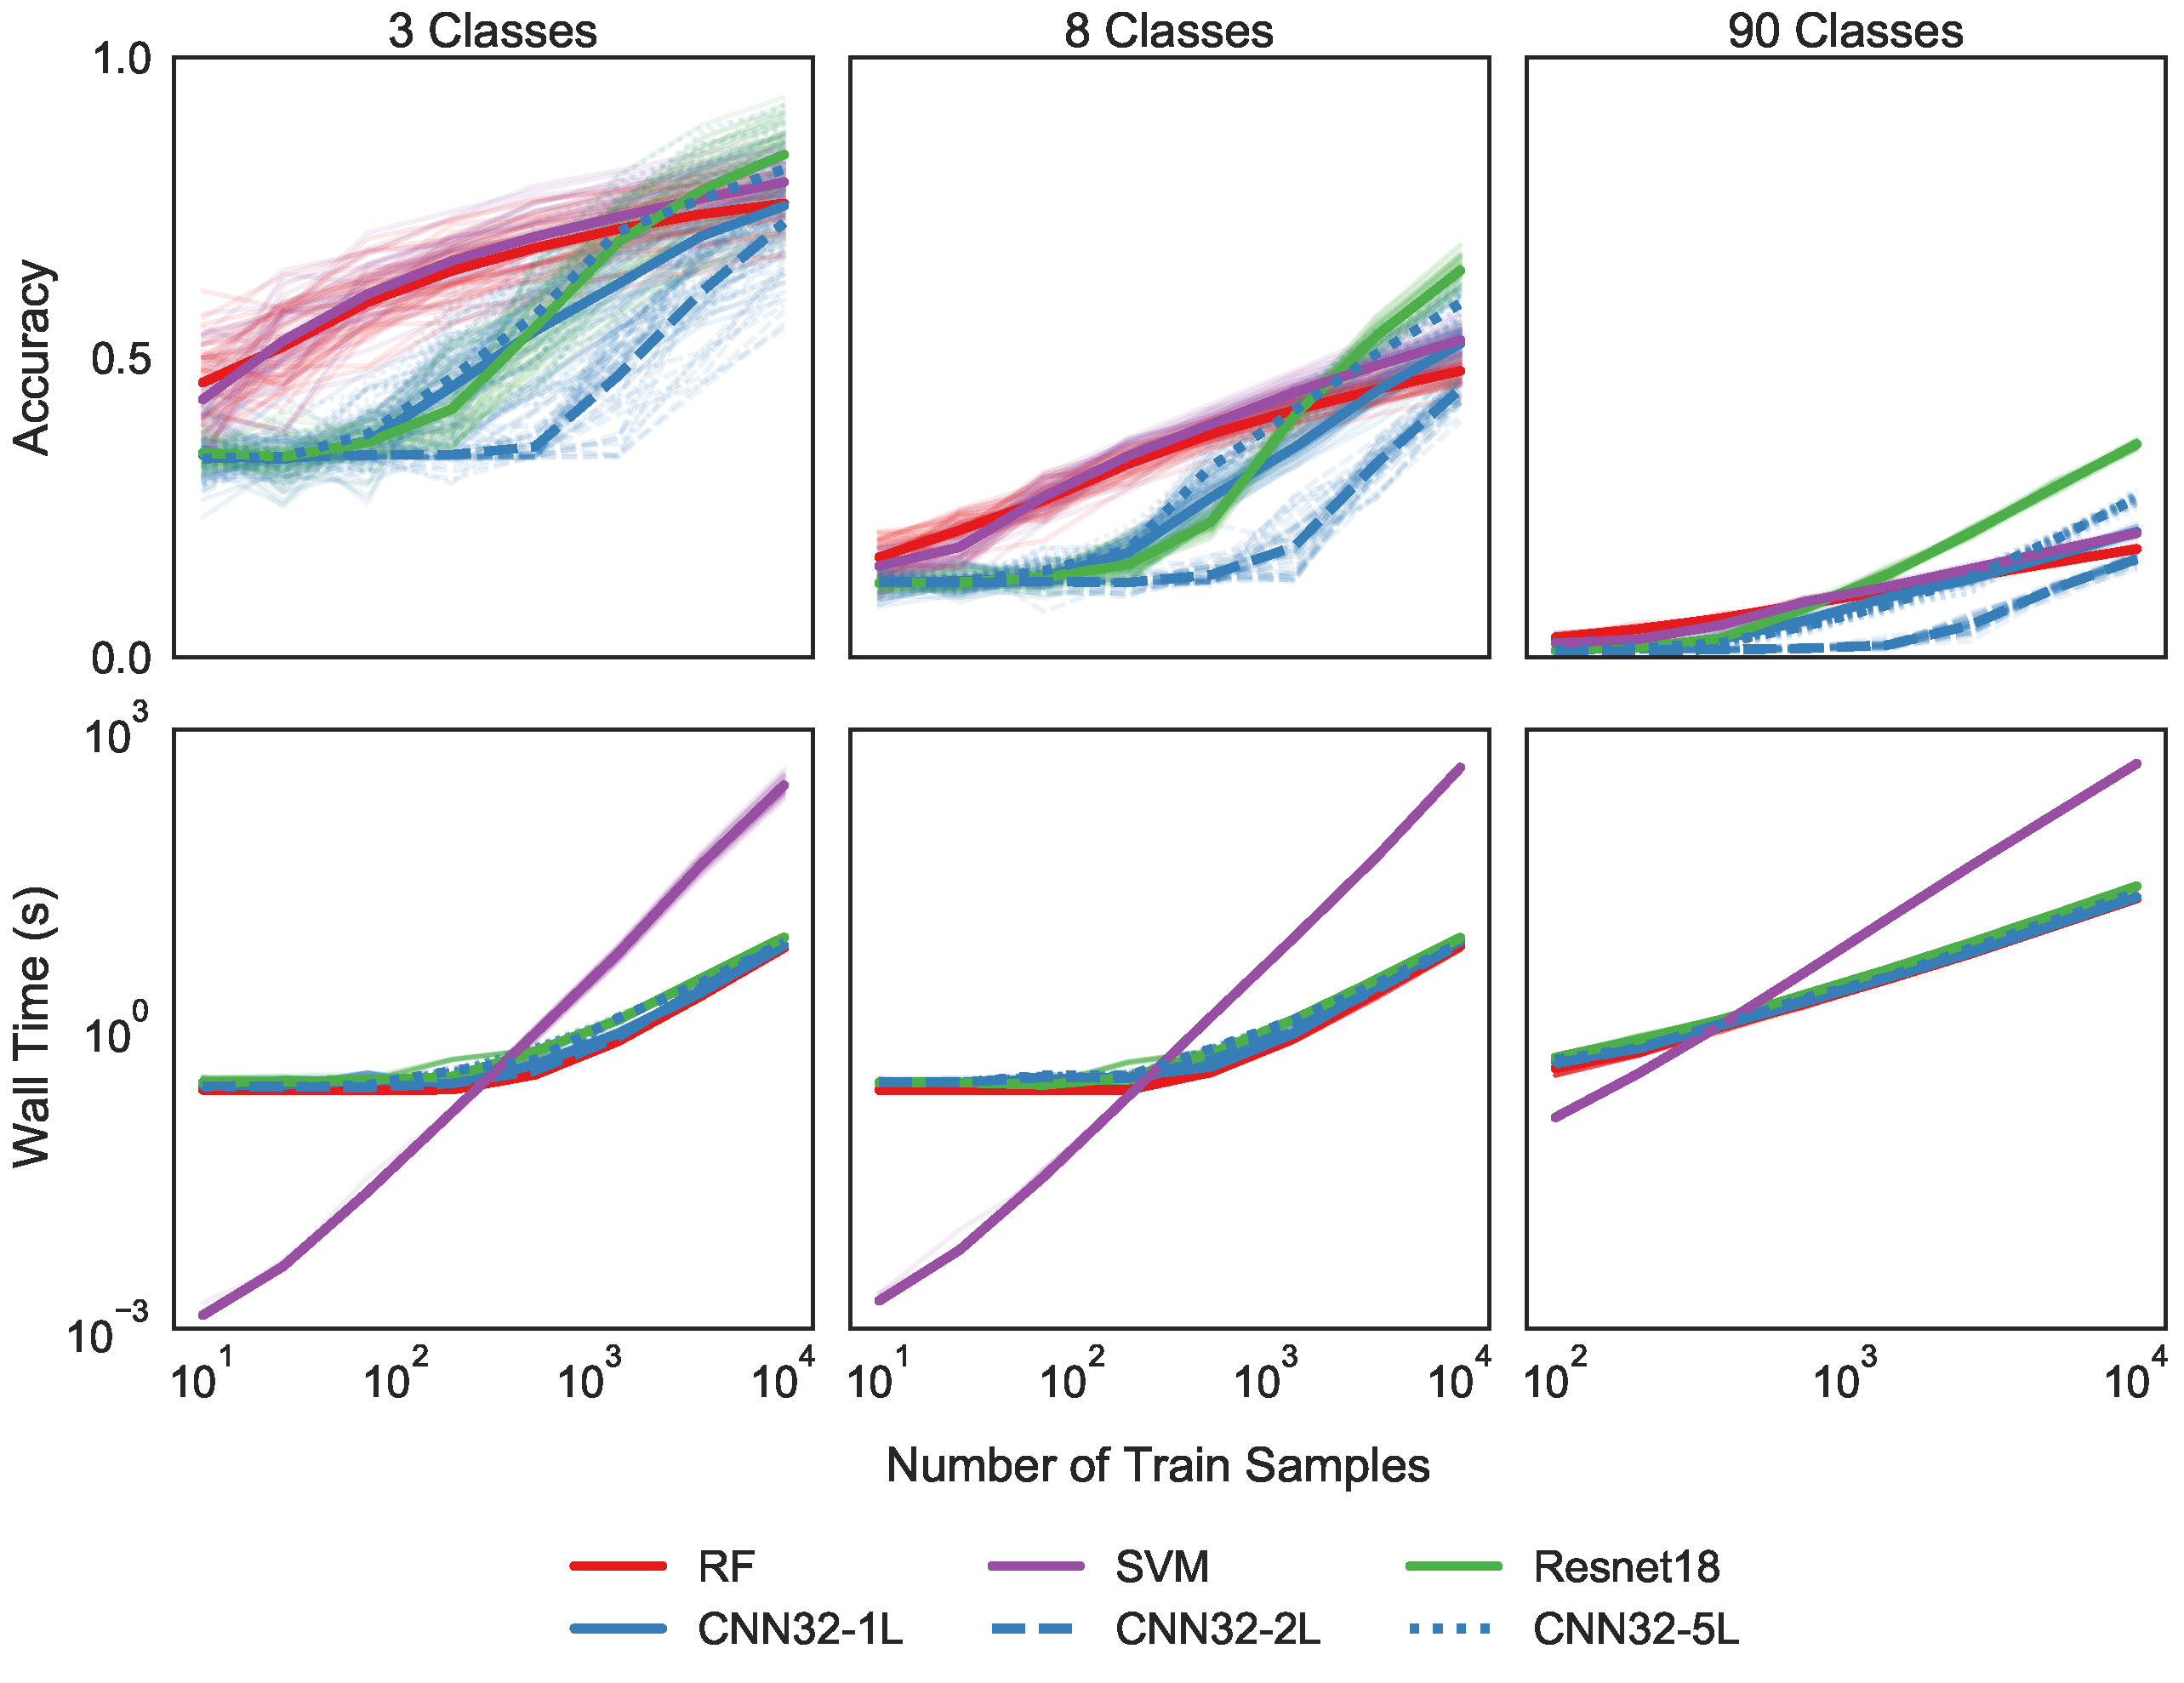
\includegraphics[width=0.8\textwidth]{figures/cifar_st.pdf}
  \caption{Performance of RF, SVM-RBF, and DN on multiclass CIFAR-10/100 classifications with fixed training time.
  Upper row represents classifier accuracy on a linear scale, and bottom row represents training wall times in seconds on a logarithmic scale. The x-axes correspond to logarithmic sample sizes for respective columns. Each panel shows average results over 45 random combinations. The left two columns use CIFAR-10, while the rightmost uses CIFAR-100.
  RF and SVM-RBF have higher classification accuracy and lower training wall times compared to CNNs at smaller sample sizes. Complex networks, however, surpass RF and SVM-RBF at larger sample sizes, and ResNet-18 always performs best in the end.
  }
\label{fig:cifar_st}
\end{figure}
\vfil\eject

Image benchmarks with the CIFAR datasets show that DN would benefit from larger sample sizes and higher class numbers. More complex networks like ResNet-18 would achieve better performance (Figure \ref{fig:cifar}). In contrast, RF and SVM-RBF maintained the advantage on classification accuracy at small sample sizes, especially when the training times were fixed (Figure \ref{fig:cifar_st}). 

\section{Audio}
\label{audio}
We performed benchmarks on the Free Spoken Digit Dataset (FSDD) (CC BY-SA 4.0) \citep{FSDD}. The dataset includes six different speakers pronouncing each of the 10 digits 50 times, for a total of 3,000 audio recordings. Similar to the image dataset analysis, we considered RF, SVM-RBF, and various CNN architectures with different layers.

\subsection{Methods}
\subsubsection{Computing}
For the 3-class and 8-class training sets, we sampled 480 recordings by selecting 45 random combinations of class labels and stratifying data equally among the classes. We also randomly selected 10\% of all the recordings for validation and another 10\% for benchmarks \citep{nasr, tian}.

To preprocess the audio files for DN, we used the short-time Fourier transform to convert the 8 kHz raw audio signals into spectrograms \citep{wyse}. In addition, we extracted mel-spectrograms (Appendix \ref{mel}) and mel-frequency cepstral coefficients (MFCC) (Appendix \ref{mfcc}) using PyTorch's inbuilt functions \citep{pytorch}.
The size of fast Fourier transforms was set to 128 for spectrograms and mel-spectrograms, and 128 coefficients were retained for MFCC. We then scaled the data to zero mean and unit variance and reshaped the results into 32x32 single-channel images \citep{lecun2012efficient}. RF and SVM-RBF treated each of the 1,024 pixel features independently of one another.

For RF and SVM-RBF, we still used \texttt{RandomForestClassifier} and \texttt{SVC} from the scikit-learn package \citep{scikit-learn}. Compared to the DN architectures for image data (Section \ref{image}), the only modification we made was setting the channel input to one for all the simpler CNNs. However, the pre-trained ResNet-18 required three channels for RGB colors. To accommodate this requirement, we concatenated the images to two duplicates of themselves along the channel dimension. This new approach would be called ResNet-18-Audio for differentiation.

All hyperparameters were the same as those of image analysis. We benchmarked the models on the same Microsoft Azure compute with a 6-core CPU and a 1-core GPU: Standard\_NC6 (Table \ref{table:azure}).

\subsubsection{Evaluation Criteria}
We evaluated the performance by classification accuracy. After training the classifiers, we benchmarked them using 10\% of the dataset that was left aside, giving us 30 audio samples per class.
Thus, the test sets for the 3-class classification task had 90 audio samples, while the 8-class test sets had 240 audio samples.

\subsection{Results}
\subsubsection{Spectrogram}
RF performed the best among all classifiers for essentially all sample sizes and all numbers of classes (Figure \ref{fig:spoken_digit}). ResNet-18-Audio had the worst performance in both tasks, presumably due to the small sample sizes that did not allow the complex network to train all its parameters effectively.
The accuracy in the 8-class task compared to 3-class was lower for all models across all sample sizes. Thus, RF excels at audio classifications for small sample sizes, while simpler DN would perform better than complex ones.
The results with mel-spectrogram (Figure \ref{fig:mel}) and MFCC (Figure \ref{fig:mfcc}) conversions were qualitatively similar.

\begin{figure}[!htb]
\centering
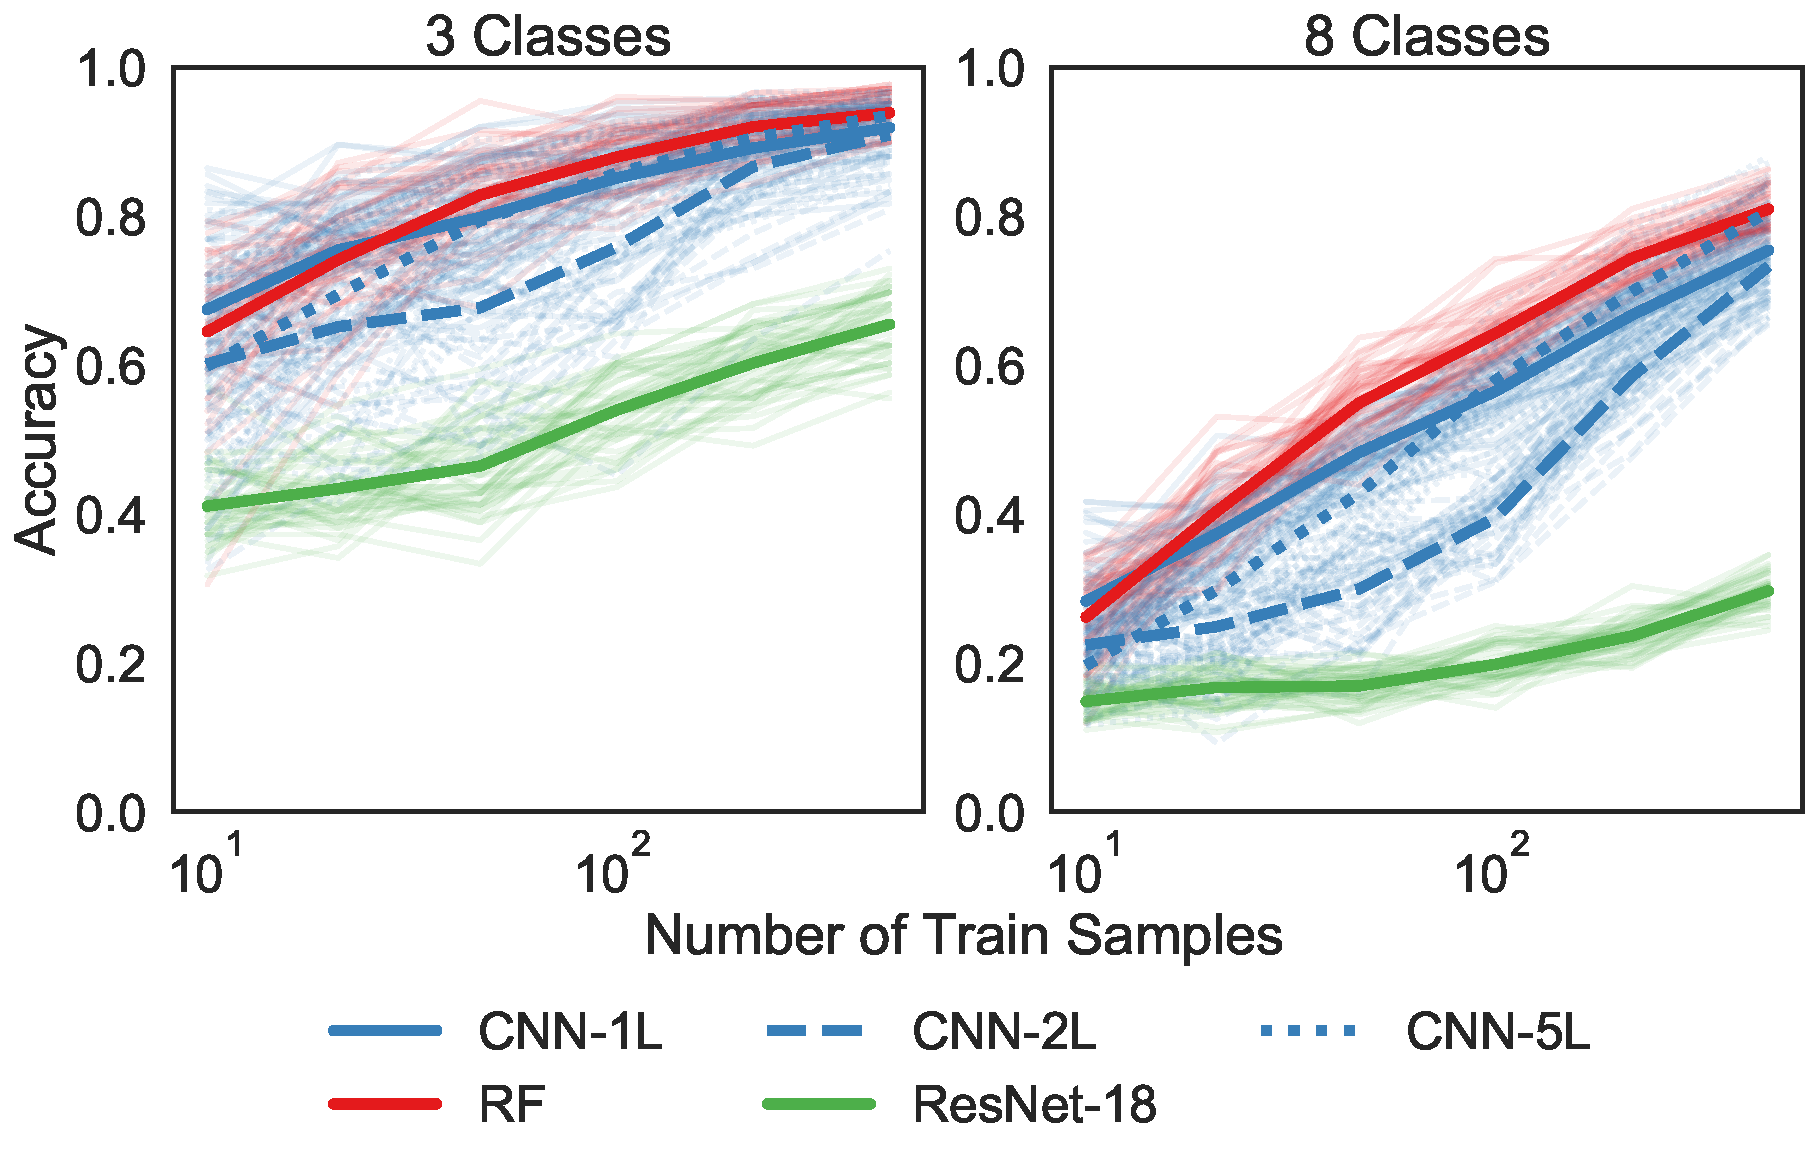
\includegraphics[width=0.6\textwidth]{figures/spoken.pdf}
  \caption{Performance of RF, SVM-RBF, and DN on multiclass FSDD classifications using spectrogram. 
  The y-axes represent classifier accuracy on a linear scale and the x-axes correspond to logarithmic sample sizes from 10 to 480. Each panel shows average results over 45 random class combinations and individual trajectories with lower alpha.
  In the 3-class task, RF, SVM-RBF, 1-layer, and 5-layer CNNs all have very similar performances. In the 8-class task, RF achieves the highest accuracy. ResNet-18-Audio performs much worse than other classifiers.
  }
\label{fig:spoken_digit}
\end{figure}
\vfil\eject

\section{Conclusion}
\label{conclusion}
We provided performance comparisons for RF and DN on three data modalities and produced consistent results. In general, we found RF to excel at tabular and structured data (image and audio) with small sample sizes, whereas DN performed better on structured data with larger sample sizes. There do exist some limitations to this technical report, which we are planning to address in the coming months. Our next steps include: adding more metrics and stratifications to results, optimizing hyperparameter search for each sample size, and including other estimators in benchmarks, such as gradient boosting trees (GBDT) and sparse projection oblique randomer forests (SPORF) \citep{gbdt, sporf}. Benchmark code will be available at GitHub: \url{https://github.com/neurodata/rf-dn-paper}.
